\documentclass[]{article}
\usepackage{atlasphysics}
% Nice maths macros
\usepackage{amsmath}
% Units
\usepackage{siunitx}
% Figures and floats
\usepackage{graphicx,subfigure,float}

% Graphics folider
\graphicspath{{figures/}}

% Scientific notation
% http://www.tapdancinggoats.com/easy-scientific-notation-in-latex.htm
\providecommand{\e}[1]{\ensuremath{\times 10^{#1}}}
% Differential Operator
\renewcommand{\d}[1]{\ensuremath{\,\operatorname{d}\!{#1}}}
% Absolute value
\renewcommand{\mod}[1]{\ensuremath{\lvert {#1} \rvert}}
% Airys functions Ai(x) and Bi(x)
\newcommand{\Ai}[1]{\ensuremath{\operatorname{Ai}({#1})}}
\newcommand{\Bi}[1]{\ensuremath{\operatorname{Bi}({#1})}}

\begin{document}

\title{Masses of S-State Quarkonium via the Roots of Airy's Function $\Ai{x}$}
\author{Alex Pearce}
\date{\today}
\maketitle


\begin{abstract}
We solve the Schr\"{o}dinger equation for $\ell = 0$ bound charm-anticharm \ccbar and bottom-antibottom \bbbar states in order to find the charm and bottom quark masses. The eigenvalues of the Hamiltonian may be found by finding the roots of Airy's functions $\Ai{x}$ and so a numerical approach, that of Ridder's method, was used to find these roots. The roots were then compared against experimentally obtained excited meson masses to find a charm mass of $m_{c} = 1.213\GeV$ and a bottom mass of $m_{b} = 4.505\GeV$. The linear radial potential $V = kr$ was found to differ slightly in strength for \ccbar and \bbbar with $\Delta k = TODO$.
\end{abstract}


\section{Introduction}\label{sec:intro}

A meson is a bound state of a quark and an antiquark. A neutral pion $\pi^{0}$ is a quantum superposition of \uubar and \ddbar, specifically $1/\sqrt{2}(\uubar + \ddbar)$. Quarkonium is an umbrella term for any meson which is comprised of a quark and its antiparticle \qqbar.\footnotemark\ A bound state of \ccbar is called charmonium and that of \bbbar is called bottomonium.

% Meson/Quarkonium distinction
\footnotetext{Note the distinction between a quark and \emph{any other} antiquark, such as $u\bar{s}$, and a quark and it's \emph{own antiparticle}, such as $\ccbar$. The latter is quarkonium, the former belongs in the broader category of mesons.}

Under the laws of QCD, we cannot observe states of colour. That is to say we can only see colourless states. Quarks and gluons (the gauge bosons of QCD), carry colour\footnotemark\ and hence cannot be observed on their own. This property of quarks and gluons is known as colour confinement. Because of colour confinement we cannot measure the quark mass directly, and so must turn to indirect methods of measurement.

% Quark and gluon colour
\footnotetext{A quark carries one colour or anticolour such as red, green or antiblue ($r$, $g$ or $\bar{b}$) whilst a gluon carries a superposition of two one colour and one anticolour states such as red-antigreen and green-antired ($1/\sqrt{2}(r\bar{g} + g\bar{r})$). For an enlightening discussion on colour theory see Griffiths~\cite{ref:dgriffithsparticles}.}

As all mesons are colourless they are, in principle, observable. (They may decay extremely quickly or be very massive making them difficult to produce and/or observe, though.) We may nav\"{i}ely think that if we can measure the masses several different mesons then we could extract the constituent quark masses from the data, but unfortunately the mass of meson is not just the sum of the `bare masses' of the quarks inside; it is this bare mass plus the binding energy between the two quarks. This leads us to conclude that if we could obtain the binding energy then we could obtain the individual quark masses.

TODO: put sections numbers in the bit below

We set out by solving the Schr\"{o}dinger equation for quarkonium to find that it's solution is Airy's function $\Ai{x}$, where the roots of this function are related to the binding energy of the \qqbar pair.

We find the roots via a numerical algorithm and then plot these roots against experimental data of meson masses in order to extract both the strength of the binding potential $V=kr$ and the charm and bottom quark masses $m_{c}$ and $m_{b}$.


\section{Solving the Schr\"{o}dinger equation for \qqbar}\label{sec:schrodinger}

We start by presuming that the bound \qqbar meson is massive enough such that we use non-relativistic quantum mechanics, hence we may employ the Schr\"{o}dinger equation. TODO: Why? We solve the time-independent radial equation as for the electron-proton bound state (i.e. the Hydrogen atom~\cite{ref:dgriffithsquantum})
\[
-\frac{\hbar^{2}}{2m}\left (
	\frac{1}{r^{2}} \frac{\d{}}{\d{r}} \left (
		r^{2} \frac{\d{\psi}}{\d{r}}
	\right )
	- \frac{\ell(\ell+1)}{r^{2}}\psi
\right )
+ V(r)\psi = E\psi.
\]
Here $m$ is the so-called reduced mass (equal to half of each constituent quark mass e.g. $m_{c}/2$ for charmonium), $\ell$ is the orbital angular momentum quantum number, $V(r)$ is the binding potential, $\psi$ is the eigenwavefunction of the Hamiltonian $H$ and $E$ is the eigenvalue for $\phi$ under $H$. Note this is, as mentioned, an eigenvalue problem $H\psi=E\psi$.

\subsection{Assumptions}\label{ssec:assumptions}

We shall investigate quarkonium states with zero angular momentum, that is $\ell = 0$. In addition, as mentioned previously, we shall work in the non-relativistic regime.

The most crucial approximation that we make is that of the binding potential $V(r)$. We shall use a linear potential model, that of $V(r) = kr$ where $k$ is some real coefficient. The value of $k$ is not known but may be deduced using the relation between meson mass and quark mass as follows.

As stated previously, we hope that the measured mass of meson of not only the mass of its constituent quarks but also includes the binding energy of the bound system (via the mass-energy equivalence $E=mc^{}2$). Then, we assume a measured meson mass conforms to
\begin{equation}\label{eqn:mesonmass}
M_{n} = 2m_{q} + E_{n}
\end{equation}
where $n$ refers to the $n$th \emph{excited state} of the meson. The excited states may be thought of like those of an electron orbiting a proton: the bound quarks may occupy infinitely many quantised energy levels of increasing radial distance and increasing energy.

Given experimental data of excited meson masses then, we can plot our binding energies $E_{n}$ against them to find the quark mass $m_{q}$.

\subsection{Manipulation}

We may work our Schr\"{o}dinger equation in to a much more manageable form. First, we apply our $\ell = 0$ assumption and make the change of variable $u = r\psi$
\[
-\frac{\hbar^{2}}{2m}
 \frac{\d{^{2}u}}{\d{r}^{2}}
+ V(r)u = Eu.
\]
After moving the $Eu$ over to the left and making one further change of variable $r = ax + b$ we  arrive at
\begin{equation}\label{eqn:airys}
\frac{\d{u}}{\d{x}} - xu = 0,
\end{equation}
where we have chosen $a = \sqrt[3]{2mk/\hbar^{2}}$ and $b = E/k$.

This is beneficial is several ways. Not only has the problem been reduced to a single order ordinary differential equation (ODE), the ODE is a well studied one that is analytically solvable. In particular, equation \ref{eqn:airys} is Airy's equation with solutions $y(x) = c\Ai{x} + d\Bi{x}$. The two solutions $\Ai{x}$ and $\Bi{x}$ are known as Airy's function. We note that as $\Bi{x}$ becomes singular as $x$ tends to infinity it is a non-physical solution and so $d = 0$. This leaves us with $\Ai{x}$ (referred to from now on as `Airy's function') as the solution to our ODE.\footnotemark
\[
y(x) = \Ai{x}
\]

\footnotetext{$\Ai{x} \to 0$ as $x \to \pm\infty$.}

\section{Approximation of \Ai{x}}\label{sec:approximation}

We require that as $r \to 0$ our wavefunction $\psi$ remains finite. As $u = r\psi$, it follows that $u \to 0$ as $r \to 0$. We must now require that $\Ai{x = 0} = 0$, i.e.\ we need to find to roots of Airy's function.

In order to do this we shall approximate Airy's function with three different representations. This is often necessary for complex analytical functions that vary there behaviour along $x$, e.g.\ changing from oscillatory to exponential, hence different expansions are favoured for different ranges in $x$.

The three approximations for Airy's function $\Ai{x}$ are given here without a full explanation of terms here, but are reproduced in term in appendix \ref{app:approximations}.

For small $\mod{x}$ we have

\begin{equation}\label{eqn:airyfirst}
\Ai{x} = 0.3550280538f(x) - 0.2588194037g(x),
\end{equation}

For larger $\mod{x}$ we may use the alternative approximations
\begin{align}\label{eqn:airysecond}
\Ai{x} \approx \frac{1}{2}\pi^{-1/2}x^{-1/4}e^{-\zeta} \sum\limits_{k=0} (-1)^{k}c_{k}\zeta^{-k},
\end{align}
and
\begin{equation}\label{eqn:airythird}
	\begin{split}
		\Ai{-x} \approx \pi^{-1/2}x^{-1/4}
		\Bigl(
			&\sin{(\zeta + \frac{\pi}{4})}\sum\limits_{k=0}(-1)^{k}c_{2k}\zeta^{-2k} -\\
			&\cos{(\zeta + \frac{\pi}{4})}\sum\limits_{k=0}(-1)^{k}c_{2k+1}\zeta^{-(2k+1)}
		\Bigr),
	\end{split}
\end{equation}

This is the Chebyshev expansion of Airy's function $\Ai{x}$~\cite{ref:agil}. The coefficients $c_{k}$ (see equation \ref{eqn:ck}) are in fact divergent, but the series expansions give good approximations up to around $k = 5$.

We will refer to equations \ref{eqn:airyfirst}, \ref{eqn:airysecond}, and \ref{eqn:airythird} and the first, second, and third approximation of Airy's function respectively (keeping in mind that each representation is appropriate for different values of $x$).

\subsection{Recursive Computation}\label{ssec:recursion}

The expressions for the series expansions coefficients $c_{k}$ in equation \ref{eqn:ck} are clearly quite cumbersome, but we may tame them to a degree via recursive computation. The functions $f(x)$ and $g(x)$ in the first approximation of $\Ai{x}$ may also be treated recursively (see equations \ref{eqn:airyfirstf} and \ref{eqn:airyfirstg}).

The advantages of recursive computation are many, but for our purposes they allow us to compute moderately small numbers that may involve large terms during computation.

For example, $f(x)$, as in equation \ref{eqn:airyfirstf}, carries a factorial in the denominator of each term. The factorial function $n!$ grows extremely rapidly with $n$,\footnotemark~ but if we note that each factorial term is simply $(n+3)!$, where $n$ is the factorial argument of the \emph{previous} term, all we have to do to find the next term is multiply the previous term by $(n+1)(n+2)(n+3)$.

\footnotetext{Interestingly, the factorial $n!$ grows even faster than the exponential function $e^{n}$.}

As the factorial is in the denominator, the final number will be small, but computing this by blindly calculating $x!$ will result in storing huge numbers in memory as the number of terms in the series increases. Modern computers can only handle numbers of a certain magnitude before they overflow, causing large numerical errors. Recursion stops the storage of large numbers in memory, preventing this problem.

The derivation of the recursive forms of $f(x)$, $g(x)$ and the coefficients $c_{k}$ are given in appendix \ref{app:recursion}. Note that $c_{k}$ benefits hugely from recursive computation as it prevents us having to calculate $216^{k}$, requiring us to merely multiply successive terms by $1/216$. 

\section{Figures}\label{sec:figures}



\appendix
\section{Approximations of \Ai{x}}\label{app:approximations}

For small $\mod{x}$ we have

\[\Ai{x} = 0.3550280538f(x) - 0.2588194037g(x),\]
where $f(x)$ and $g(x)$ are infinite series given by
\begin{align}
f(x) &= 1 + \frac{1}{3!}x^{3} + \frac{1\times4}{6!}x^{6} + \frac{1\times4\times{7}}{9!}x^{9} + \dotsb,\label{eqn:airyfirstf}\\
g(x) &= x + \frac{2}{4!}x^{4} + \frac{2\times5}{7!}x^{7} + \frac{2\times5\times{8}}{10!}x^{10} + \dotsb\label{eqn:airyfirstg}.
\end{align}

For larger $\mod{x}$ we may use the alternative approximations
\[
\Ai{x} \approx \frac{1}{2}\pi^{-1/2}x^{-1/4}e^{-\zeta} \sum\limits_{k=0} (-1)^{k}c_{k}\zeta^{-k},
\]
and
\[
	\begin{split}
		\Ai{-x} \approx \pi^{-1/2}x^{-1/4}
		\Bigl(
			&\sin{(\zeta + \frac{\pi}{4})}\sum\limits_{k=0}(-1)^{k}c_{2k}\zeta^{-2k} -\\
			&\cos{(\zeta + \frac{\pi}{4})}\sum\limits_{k=0}(-1)^{k}c_{2k+1}\zeta^{-(2k+1)}
		\Bigr),
	\end{split}
\]
where
\begin{equation}\label{eqn:ck}
c_{k} = \frac{(2k+1)(2k+3)\dotsb(6k-1)}{216^{k}k!} = 1,
\end{equation}
with $c_{0} = 1$. Lastly
\[
\zeta = \frac{2}{3}x^{3/2}.
\]

\subsection{Recursive Representation}\label{app:recursion}

After some algebra, the functions $f(x)$ and $g(x)$ in the first approximation of $\Ai{x}$ may be represented recursively. The $n$th term in each series are then
\begin{align*}
f_{n}(x) &= \frac{f_{n-1}(x)}{(3n^{2} - n)} \frac{x^{3}}{3},\\ 
g_{n}(x) &= \frac{g_{n-1}(x)}{(3n^{2} + n)} \frac{x^{3}}{3},
\end{align*}
where $f_{0}(x) = 1$ and $g_{0}(x) = x$.

The series coefficients $c_{k}$ used in the second and third approximations of $\Ai{x}$ may also be presented recursively. TODO: this.
\[
c_{k} = 1
\]

\begin{figure}[H]
	\hspace*{-0.15\textwidth}
	\centering
	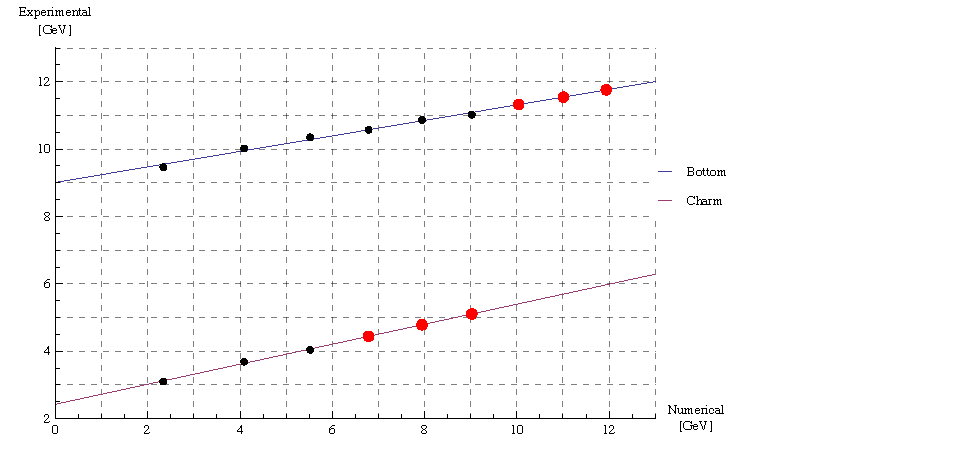
\includegraphics[scale=1.3]{experimental-numerical}
	\caption{TODO: Caption here}
	\label{fig:data}
\end{figure}


\begin{thebibliography}{9}
	\bibitem{ref:iaitchison}
	I. J. R. Aitchenson \& A. J. G. Hey,
	\emph{Gauge Theories in Particle Physics, Volume II: QCD and the Electroweak Theory},
	Institute of Physics Publishing, Bristol, UK,
	3rd Edition,
	2003.
	

	\bibitem{ref:gdaniell}
  G. J. Daniell,
  \emph{PHYS6017 Course Notes},
  University of Southampton, Southampton, UK,
  2011.
  
	\bibitem{ref:agil}
  A. Gil, J. Segura and N. M. Temme,
  \emph{Numerical Methods for Special Functions},
  Society for Industrial and Applied Mathematics, Philadelphia PA, USA,
  $1$st Edition,
  2007.
  
   \bibitem{ref:dgriffithsparticles}
  D. Griffiths,
  \emph{Introduction to Elementary Particles},
  Wiley-VCH, Weinheim,
  2nd Edition,
  2003.
  
  \bibitem{ref:dgriffithsquantum}
  D. Griffiths,
  \emph{Introduction to Quantum Mechanics},
  Wiley-VCH, Weinheim,
  6th Edition,
  2011.
  
  \bibitem{ref:nr}
  W. H. Press et al.,
  \emph{Numerical Recipes: The Art of Scientific Computing},
  Cambridge University Press, Cambridge, UK,
  $3$rd Edition,
  2007.
  
  \bibitem{ref:mvoloshin}
  M.B. Voloshin,
  ``Charmonium'',
  \emph{Prog.\ Part.\ Nucl.\ Phys.\ } \textbf{61},
  Issue 2,
  p455-511 (2008).
  
\end{thebibliography}

\end{document}